\documentclass[a4paper]{article}

\usepackage[english]{babel}
\usepackage{amsmath}
\usepackage{amssymb}
\usepackage{dsfont}
\usepackage{tikz}
\usepackage{framed} 
\usetikzlibrary{arrows,automata}
\title{Calculus and Probability Theory\\ Assignment 6}
\author{Christoph Schmidl\\
s4226887\\
Data Science\\
c.schmidl@student.ru.nl\\}
\date{\today}


\begin{document}
\maketitle





\textbf{After completing these exercises successfully you should be confident with the following topics:}

\begin{itemize}
	\item compute combinatorial problems
	\item recognize the birthday paradox
	\item work with the basic definitions of probability theory
\end{itemize}
\vspace{1em}

\begin{enumerate}


%%%%%%%%%%%% Task 1 %%%%%%%%%%%%
\item (\textbf{10 points}) Vanessa wants to give her friend potted plants as present. At the local florist, the flowers come in five colors, and there are four types of flower pots.


\begin{enumerate}
	%%%%%%%% Task 1.a %%%%%%%%
	\item If Vanessa buys one potted flower (any combination of a flower and a pot), how many different options can Vanessa choose from?\\
	\textbf{Solution:}\\
	
	
Flower Colors available: 5\\
Flower Pots available: 4\\

All available combinations: $5 \cdot 4 = 20$\\	
	
	
	
	%%%%%%%% Task 1.b %%%%%%%%
	\item If Vanessa buys two potted flowers and she wants two different combinations, how many options does she have? (Two combinations are different if at least the colors of the flowers or the types of the pots are different.)
	\textbf{Solution:}\\
	
	
	
	
	
	
	
	
The first choice of a potted flower is freely choosable, therefore 20 combinations at that point.\\

The second choice of a potted flower is now restricted by the one which was chosen before. Therefore, there are now $20 - 1 = 19$ combinations left.\\

Overall, she has $20 \cdot 19 = 380$ options to choose from.\\



	
\end{enumerate}



%%%%%%%%%%%% Task 2 %%%%%%%%%%%%
\item (\textbf{5 points}) In how many ways can five out of eight people be seated on a sofa if there are only five seats available?\\
\textbf{Solution:}\\

We have $n = 8$ from which we take samples of size $r = 5$. The order on the seated people on the sofa matters and people who are already seated cannot be seated again. Therefore, no replacement.\\

Number of options: $\frac{8!}{(8 - 5)!} = 8 \cdot 7 \cdot 6 \cdot 5 \cdot 4 = 6720$

Five out of eight people can be seated on a sofa in 6720 ways if there are only five seats available.\\




%%%%%%%%%%%% Task 3 %%%%%%%%%%%%
\item (\textbf{5 points}) Three cards are drawn at random (without replacement) from an ordinary deck of 52 cards. Find the number of ways in which one can draw



\begin{enumerate}
	%%%%%%%% Task 3.a %%%%%%%%
	\item a diamond and a club and a heart in this order\\
	\textbf{Solution:}\\
	
We have 13 ways to draw a diamond from the whole suit of diamonds available. The same goes for the club and the heart. Therefore, we have $13 \cdot 13 \cdot 13 = 2197$ ways to draw a diamond and a club and a heart in succession.\\	
	
	
	
	%%%%%%%% Task 3.b %%%%%%%%
	\item one heart and then two clubs or two spades\\
	\textbf{Solution:}\\
	
There are 13 ways to draw one heart out of the suit in the beginning.\\

To draw one club or a spade, there are 26 ways. As soon as we draw the club or the spade, we are left with 12 ways, because we already draw one card of the suit and at this point we are bound to either club or spade.\\
Therefore, there are $13 \cdot 26 \cdot 12 = 4056$ ways to draw one heart and then two clubs or two spades.\\

Another way to look at the problem:

13 ways do draw one heart out of the suit in the beginning. After that, we have $13 \cdot 12 = 156$ ways to draw two clubs or $13 \cdot 12 = 156$ ways to draw two clubs. Therefore, $13 \cdot 2(13 \cdot 12) = 4056$\\




	
\end{enumerate}




%%%%%%%%%%%% Task 4 %%%%%%%%%%%%
\item (\textbf{10 points}) How many numbers, consisting of five different digits each, can be made from the digits 1,2,3,...,9 if


\begin{enumerate}
	%%%%%%%% Task 4.a %%%%%%%%
	\item the numbers must be even?\\
	\textbf{Solution:}\\




A number is even, if it ends with the digit 2,4,6 or 8.\\
Let's start from the end of the five digit number. Because the number has to end with 2,4,6 or 8, we have 4 possibilities to choose from.\\

After that, we can choose from the whole range of the given digits and decrement the number of possibilites after we've chosen the next digit.\\

Therefore, there are $4 \cdot 8 \cdot 7 \cdot 6 \cdot 5 = 6720$ numbers.\\

	
	%%%%%%%% Task 4.b %%%%%%%%
	\item exactly two of the digits are odd?\\
	\textbf{Solution:}\\
	
An odd digit is 1,3,5,7 or 9. Therefore, there are 5 ways to choose an odd digit. Because we are free to choose our placement of an odd digit in the beginning and there are 5 digit placements to choose from, we have $5 \cdot 5 = 25$ options in the beginning.\\

After that, we are left with 4 digit placements and 4 digits to choose from. Therefore, $4 \cdot 4 = 16$ options to choose our second odd digit. So, we have $25 \cdot 16 = 400$ ways for the placement of two odd digits, which are different. After that, we are still left with 3 digits. We can choose from 7 options for the third digit, then 6 options for the fourth and 5 options for the fifth.\\

In the end, we have $25 \cdot 16 \cdot 7 \cdot 6 \cdot 5 = 84000$ ways to choose a number, consisting of five different digits each and where exactly two of the digits are odd.\\


	
	
	%%%%%%%% Task 4.c %%%%%%%%
	\item How many numbers are in (a) and (b) if repetitions of the digits are allowed?\\
	\textbf{Solution:}\\


This question is unclear. You can interpret it as follows:

\begin{itemize}
	\item Answer (a) and (b) again with the condition that repetitions of digits are allowed\\
	\textbf{Solution:}\\
	
	(a) $9^4 \cdot 4 = 26244$\\
	(b)	$5^2 \cdot 9^3 = 18225$\\
	
\end{itemize}	

Or 
	
\begin{itemize}
	\item How many numbers share the property of (a) and (b) with the condition that repetition of digits is allowed?\\
	\textbf{Solution:}\\
	
	$4 \cdot (5 \cdot 4) \cdot (5 \cdot 3) \cdot 9 \cdot 9 = 97200$\\
\end{itemize}		
	
	
\end{enumerate}



%%%%%%%%%%%% Task 5 %%%%%%%%%%%%
\item (\textbf{10 points}) According to Wikipedia a new scheme was introduced for license plates in the Netherlands. The short summary of the scheme is shown below. In practice, some letters are excluded to avoid confusion and obscene language; however, \textit{we ignore this} in this exercise!\\
Answer the following questions and give brief explanations.

\begin{figure}[ht!]
	\centering
  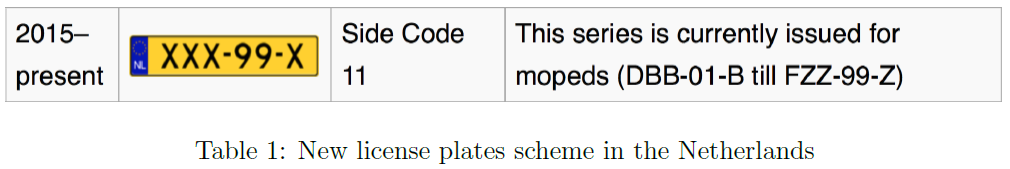
\includegraphics[width=0.8\textwidth]{license.PNG}
\end{figure}	



\begin{enumerate}
	%%%%%%%% Task 5.a %%%%%%%%
	\item Consider only the image in the second entry of the table above. How many possible license plates can be made with this setup. (We assume that 26 letters can be used where X is displayed, and 10 digits can be used where 9 is displayed.)\\
	\textbf{Solution:}


\begin{align}
26 \cdot 26 \cdot 26 \cdot 10 \cdot 10 \cdot 26 = 45697600\notag
\end{align}

	
	%%%%%%%% Task 5.b %%%%%%%%
	\item In the fourth column of Table 1 a range is provided for mopeds. (Note that it is a range, so for example \textbf{EAA-01-A is in the range!}) Using this, count how many license plates can be issued for mopeds?\\
	\textbf{Solution:}

\begin{align}
(3 \cdot 26 \cdot 26 \ 10 \cdot 10 \cdot 26) - (26 \cdot 10 \cdot 10 + 1) = 5272800 - 2601 = 5270199\notag
\end{align}

I calculated the range from DAA-00-A to FZZ-99-Z and then substracted the range DAA-00-A tp DBB-00-B.\\

	
	%%%%%%%% Task 5.c %%%%%%%%
	\item Assuming that there are only cars and mopeds in this scheme, can you tell what kind of vehicle has the license plate \textbf{DFA-78-V}? And \textbf{DAF-78-A}? and \textbf{DCF-78-V}?\\
	\textbf{Solution:}\\	
	
\textbf{DFA-78-V}: Moped\\
\textbf{DAF-78-A}: Car\\
\textbf{DCF-78-V}: Moped\\

	
	
	%%%%%%%% Task 5.d %%%%%%%%
	\item Assuming that there are only cars and mopeds in this scheme, how many cars can be with this type of a license plate?\\
	\textbf{Solution:}	

\begin{align}
45697600 - 5270199 = 40427401\notag
\end{align}




\end{enumerate}


%%%%%%%%%%%% Task 6 %%%%%%%%%%%%
\item (\textbf{10 points}) Expand the following expressions, either directly or via binomial coefficients. Make it clear how you proceed.\\

Binomial Coefficient

\begin{align}
	{n \choose r} = \frac{n!}{r!(n - r)!}\notag
\end{align}


For arbitrary $n \in \mathbb{N}$

\begin{align}
	(x+y)^n = \sum_{i=0}^{i=n}{n \choose i}x^{n-i}y^i\notag
\end{align}





\begin{enumerate}
	%%%%%%%% Task 6.a %%%%%%%%
	\item $(x-7)^3$\\
	\textbf{Solution:}\\

\begin{align}
(x-7)^3 &= {3 \choose 0}x^3 \cdot (-7)^0 + {3 \choose 1}x^2 \cdot (-7)^1 + {3 \choose 2}x^1 \cdot (-7)^2 + {3 \choose 3}x^0 \cdot (-7)^3\notag\\
&= x^3 - 21x^2 + 147x - 343\notag
\end{align}



	%%%%%%%% Task 6.b %%%%%%%%
	\item $(x+2y)^4$\\
	\textbf{Solution:}\\
	
\begin{align}
(x+2y)^4 &= {4 \choose 0}x^4 \cdot (2y)^0 + {4 \choose 1}x^3 \cdot (2y)^1 +{4 \choose 2}x^2 \cdot (2y)^2 + {4 \choose 3}x^2 \cdot (2y)^3\notag\\ &+ {4 \choose 4}x^1 \cdot (2y)^4\notag\\
&= x^4 + 8x^3y + 24x^2y^2 + 32xy^3 + 16y^4\notag
\end{align}	
	
	
	%%%%%%%% Task 6.c %%%%%%%%
	\item $(x^3-3)^4$\\
	\textbf{Solution:}\\
	
\begin{align}
(x^3-3)^4 &= {4 \choose 0}(x^3)^4 \cdot (-3)^0 + {4 \choose 1}(x^3)^3 \cdot (-3)^1 + {4 \choose 2}(x^3)^2 \cdot (-3)^2\notag\\ &+ {4 \choose 3}(x^3)^1 \cdot (-3)^3 + {4 \choose 4}(x^3)^0 \cdot (-3)^4\notag\\
&= x^{12} - 12x^9 + 54x^6 - 108x^3 + 81\notag
\end{align}	
	
\end{enumerate}


%%%%%%%%%%%% Task 7 %%%%%%%%%%%%
\item (\textbf{5 points}) Consider a team of 11 players wishing each other luck before a match. If everyone shakes everyone else's hand exactly once, how many handshakes occur?\\
\textbf{Solution:}\\

We can choose anyone of the 11 people to shake one's hand of one of the other 10 people. But because a handshake between person a and person b is the same as a handshake between person b and person a, we have to divide the whole number by 2.

\begin{align}
	\frac{11 \cdot 10}{2} = 55\notag
\end{align}

Therefore, 55 handshakes occur.\\


%%%%%%%%%%%% Task 8 %%%%%%%%%%%%
\item (\textbf{5 points}) From four consonants and five vowels, how many six-letter words can be formed consisting of three different consonants and three different vowels? The words need not have a meaning.\\
\textbf{Solution:}\\

The number of ways to choose 3 different consonants out of 4 is ${4 \choose 3} = 4$\\

The number of ways to choose 3 different vowels out of 5 is ${5 \choose 3} = 10$\\

The number of ways to choose 3 different consonants and 3 different vowels is $4 \cdot 10 = 40$\\

Finally, these 6 letters can be arranged in $6!$ ways, therefore the total number of different words is $7! \cdot 40 = 201600$\\




%%%%%%%%%%%% Task 9 %%%%%%%%%%%%
\item (\textbf{5 points}) A school has four math teachers, three English teachers and three IT teachers. From this whole group, a five teacher committee has to be established. Calculate the number of ways that this committee can be formed if at least one IT teacher must be on the committee.\\
\textbf{Solution:}\\


Math teachers: 4\\
English teachers: 3\\
IT teachers: 3\\
Total number of teachers: 10\\

We have 5 slots to fill for this commitee. One slot has to be filled by one IT teacher, which gives us 3 possibilities to choose from in the beginning. After that, we are free to fill the 4 remaining slots with the remaining 9 teachers.\\
Therefore,

\begin{align}
 3 \cdot {9 \choose 4} = 3 \cdot \frac{9!}{4!(9-4)!} = 3 \cdot 126 = 379\notag
\end{align}

There are 379 ways to form such a committee.\\

%%%%%%%%%%%% Task 10 %%%%%%%%%%%%
\item (\textbf{10 points}) There are twelve provinces in the Netherlands. Suppose that the birth of Dutch people is uniformly distributed over all twelfe provinces, i.e. for every province $\frac{1}{12}$ of the population is born there. What is the probability that at least two of $r$ randomly selected Dutch-born people were born in the same province, where $r = 1$, $r = 2$, $r = 3$, $r = 4$, $r = 5$ or $r = 6$\\
\textbf{Solution:}\\

$n = 12$\\

We look at samples of $r$, which are ordered, with replacement (the province can occur more than once as the birth place)\\


$n^r = 12^r$ options for $r$ people.\\

Number of options: $12 \cdot 11 ... (12 - r) = \frac{12!}{(12-r)!} = {12 \choose r}r!$	
	
The probability that $r$ people are born in different provinces in the Netherlands is 

\begin{align*}
	\frac{\frac{12!}{(12-r)!}}{12^r} = \frac{12!}{(12-r)! \cdot 12^r}
\end{align*}	

Therefore, the probability that at least 2 of $r$ randomly selected Dutch-born people were born in the same province is 

\begin{align*}
p(r) = 1 - \frac{12!}{(12-r)! \cdot 12^r}
\end{align*}
	

$p(1) = 1 - \frac{12!}{11! \cdot 12} = 0$\\
$p(2) = 1 - \frac{12!}{10! \cdot 12^2} = \frac{1}{12}$\\
$p(3) = 1 - \frac{12!}{9! \cdot 12^3} = \frac{17}{72} $\\
$p(4) = 1 - \frac{12!}{8! \cdot 12^4} = \frac{41}{96}$\\
$p(5) = 1 - \frac{12!}{7! \cdot 12^5} = \frac{89}{144}$\\
$p(6) = 1 - \frac{12!}{6! \cdot 12^6} = \frac{1343}{1728}$\\








%%%%%%%%%%%% Task 11 %%%%%%%%%%%%
\item (\textbf{10 points}) We toss a coin twice.\\


\begin{enumerate}
	\item Give a corresponding sample space $S$.\\
	\textbf{Solution:}\\
	
T = Tails\\
H = Heads\\

$S = \{TT,HH,TH,HT\}$\\	
	
	
	
	\item Give the set of outcomes corresponding to each of the following events:
	\begin{itemize}
		\item[i] A: "we throw heads exactly one".\\
		\textbf{Solution:}

\begin{align}
	A = \{ TH,HT\}\notag
\end{align}		
		
		
		\item[ii] B: "we throw heads at least once".\\
		\textbf{Solution:}
		
\begin{align}
	B = \{ TH,HT,HH\}\notag
\end{align}				
		
		
		\item[iii] C: "tails did not appear before a head appeared".\\
		\textbf{Solution:}\\
			
		
\begin{align}
	C = \{ HH, HT, TT\}\notag
\end{align}			
		
	\end{itemize}		
	
	\item Give a probability measure $P_1$ for the sample space $S$.\\
	\textbf{Solution:}\\
	
\begin{align}
	TT = \frac{1}{2} \cdot \frac{1}{2} = \frac{1}{4} = 0.25 = 25\%\notag\\
	HH = \frac{1}{2} \cdot \frac{1}{2} = \frac{1}{4} = 0.25 = 25\%\notag\\
	TH = \frac{1}{2} \cdot \frac{1}{2} = \frac{1}{4} = 0.25 = 25\%\notag\\
	HT = \frac{1}{2} \cdot \frac{1}{2} = \frac{1}{4} = 0.25 = 25\%\notag
\end{align}	
	
There was no information if the coin was biased or the order of the sample space matters. I assume, that HT is not the same as TH!\\	
	
	
\end{enumerate}

%%%%%%%%%%%% Task 12 %%%%%%%%%%%%
\item (\textbf{5 points}) Let $P$ be a probability measure on space $S$. Prove that $P(\emptyset) = 0$\\
\textbf{Solution:}\\

A probability measure $P$ for a sample space $S$ is a function that gives for each event $A \subseteq S$ a probability $P(A) \ in [0,1]$ with

\begin{itemize}
	\item Axiom 1: $P(S) = 1$
	\item Axiom 2: for mutually exclusive events $A,B \subseteq S$, $P(A \cup B) = P(A) + P(B)$
\end{itemize}

If $P(S) = 1$, then $P(\emptyset) = 0$, because $P(S \cup \emptyset) = P(S) + P(\emptyset) = 1 + 0 = 1 \rightarrow P(\emptyset) = 0$\\





%%%%%%%%%%%% Task 13 %%%%%%%%%%%%
\item (\textbf{bonus, +5 points}) Let $P$ be a probability measure on space $S$. Prove that for pairwaise mtutally exclusive events $A_1, A_2,...,A_n$ (i.e. $A_i \cap A_j = \emptyset$ for all $i \neq j$ and $n \geq 2$) one has $P(A_1 \cup A_2 \cup ... \cup A_n) = P(A_1) + P(A_2) + ... + P(A_n).$ (Hint: use induction.)\\
\textbf{Solution:}\\




%%%%%%%%%%%% Task 14 %%%%%%%%%%%%F
\item (\textbf{10 points}) An experiment consists of drawing 3 cards in succession from a well-shuffled ordinary deck of cards. Let $A_1$ denote the event "Ace on first draw", $A_2$ the event "Ace on second draw" and $A_3$ the event "Ace on third draw". State in words the meaning of each of the following probabilites.\\


\begin{enumerate}
	\item $P(A_1 \cap \neg A_2)$\\
	\textbf{Solution:}\\
	
The probability to draw an Ace on the first and to draw no Ace on second draw.\\
You can also say: The probability to draw an Ace on the first draw and to draw anything else except an Ace on the second draw.\\	
	
	
	\item $P(A_1 \cup A_2)$\\
	\textbf{Solution:}\\
	
The probability to draw an Ace on the first draw or an Ace on second draw.\\	
	
	
	
	\item $P(\neg A_1 \cap \neg A_2 \cap \neg A_3)$\\
	\textbf{Solution:}\\
		
The probability to draw no Ace on first draw and no Ace on second draw and no Ace on third draw.\\
You can also say: The probability to draw anything in the first three draws except aces.\\	
	
	\item $P\left[ (A_1 \cap \neg A_2)\cup (\neg A_2 \cap A_3) \right]$\\
	\textbf{Solution:}\\
	
The probability to draw an ace on first draw and no Ace on second draw or to draw no ace on second draw and an ace on third draw.\\	
	
	
\end{enumerate}

\end{enumerate}

\end{document}
